\documentclass[a4paper]{article}
\usepackage[spanish]{babel}
\usepackage[utf8]{inputenc}
\usepackage{graphicx}
\usepackage{enumerate}
\usepackage{listings}
\usepackage{color}
\usepackage{indentfirst}
\usepackage{fancyhdr}
\usepackage{latexsym}
\usepackage[colorlinks=true, linkcolor=black]{hyperref}
%\usepackage{makeidx}
%\usepackage{float}
\usepackage{wrapfig}
\usepackage{calc}
\usepackage{amsmath, amsthm, amssymb}
\usepackage{amsfonts}
%\lstset{language=C}
\definecolor{gray}{gray}{0.5}
\definecolor{light-gray}{gray}{0.95}
\definecolor{orange}{rgb}{1,0.5,0}

\usepackage{fancyhdr}
\pagestyle{fancy}

%\renewcommand{\chaptermark}[1]{\markboth{#1}{}}
\renewcommand{\sectionmark}[1]{\markright{\thesection\ - #1}}

\fancyhf{}

\fancyhead[LO]{Sección \rightmark} % \thesection\ 
\fancyfoot[LO]{\small{Axel Straminsky, Jorge Quintana, Florencia Zanollo, Luis Toffoletti}}
\fancyfoot[RO]{\thepage}
\renewcommand{\headrulewidth}{0.5pt}
\renewcommand{\footrulewidth}{0.5pt}
\setlength{\hoffset}{-0.8in}
\setlength{\textwidth}{16cm}
%\setlength{\hoffset}{-1.1cm}
%\setlength{\textwidth}{16cm}
\setlength{\headsep}{0.5cm}
\setlength{\textheight}{25cm}
\setlength{\voffset}{-0.7in}
\setlength{\headwidth}{\textwidth}
\setlength{\headheight}{13.1pt}

\renewcommand{\baselinestretch}{1.1}  % line spacing
% \setcounter{secnumdepth}{2}
\usepackage{underscore}
\usepackage{caratula}
\usepackage{url}
\usepackage{float}
\usepackage{algorithm}
\usepackage[noend]{algpseudocode}





\newcommand{\cod}[1]{{\tt #1}}
\newcommand{\negro}[1]{{\bf #1}}
\newcommand{\ital}[1]{{\em #1}}
\newcommand{\may}[1]{{\sc #1}}
\newcommand{\tab}{\hspace*{2em}}

\hypersetup{
	pdfstartview= {FitH \hypercalcbp{\paperheight-\topmargin-1in-\headheight}},
	pdfauthor={Grupo},
	pdfsubject={Dise\~{n}o}
}

\lstdefinestyle{customc}{
	backgroundcolor=\color{light-gray},
	belowcaptionskip=1\baselineskip,
	breaklines=true,
	numbers=left,
	xleftmargin=\parindent,
	language=C,
	showstringspaces=false,
	basicstyle=\footnotesize\ttfamily,
	keywordstyle=\bfseries\color{blue},
	commentstyle=\itshape\color{gray},
	identifierstyle=\color{black},
	stringstyle=\color{orange},
}

\lstdefinestyle{customasm}{
	backgroundcolor=\color{light-gray},
	belowcaptionskip=1\baselineskip,
	numbers=left,
	xleftmargin=\parindent,
	language=[x86masm]Assembler,
	keywordstyle=\bfseries\color{blue},
	basicstyle=\footnotesize\ttfamily,
	commentstyle=\itshape\color{gray},
}

\lstset{escapechar=@}


\begin{document}
	
	\thispagestyle{empty}
	\materia{Teoría de las Comunicaciones}
	\submateria{Segundo Cuatrimestre de 2016}
	\titulo{TP 1: Wiretapping}
	%\subtitulo{Scheduling}
	\integrante{Axel Straminsky}{769/11}{axelstraminsky@gmail.com}
	\integrante{Jorge Quintana}{}{jorge.quintana.81@gmail.com}
	\integrante{Florencia Zanollo}{934/11}{florenciazanollo@gmail.com}
	\integrante{Luis Toffoletti}{827/11}{luis.toffoletti@gmail.com}
	
	\makeatletter
	
	\maketitle
	\newpage
	
	\thispagestyle{empty}
	\vfill
	
	\thispagestyle{empty}
	\vspace{3cm}
	\tableofcontents
	\newpage
	
	\newenvironment{myindentpar}[1]
	{\begin{list}{1}
			{\setlength{\leftmargin}{#1}}
			\item[]
		}
		{\end{list} }
	
	%\normalsize
	\newpage
	
	% -------------------------------------------------------
	% Breve explicacion de la base teorica que fundamenta los metodos involucrados en el trabajo, junto con los metodos mismos.  
	% -------------------------------------------------------
	\section{Introducción}


%El objetivo de este trabajo es analizar diversos aspectos de una red como su topología, y otros aspectos más teóricos como la entropía y la información de cada nodo. Para realizar este análisis modelamos los paquetes capturados como dos fuentes de memoria nula $S$ y $S1$, las cuáles tienen como símbolos los paquetes ARP broadcast y unicast, en el caso de $S$, y las direcciones IP de destino de estos paquetes en el caso de $S1$.

El objetivo del presente trabajo es descubrir la topología de distintas redes utilizando captura de paquetes ARP. Para la clasificación de los datos así obtenidos se modelaran por cada red dos fuentes de memoria nula, que identificaremos como $S$ y $S1$. Para las fuentes $S$ se distinguirán los paquetes broadcast vs. los paquetes unicast y para las fuentes $S1$ los símbolos se distinguirán basados en las direcciones IP de los orígenes de los paquetes ''Who-Has'' ARP.\\

ARP es un protocolo de capa 2.5 que se encarga de traducir direcciones IP (Nivel de red) a direcciones físicas de los dispositivos o ''MAC addresses'' (Nivel de Enlace). Este protocolo distingue dos tipos de mensajes, ''Who has'' e ''Is At''.\\
''Who has'' son típicamente mensajes de ''pedido'' (request) enviados a toda la red (Broadcast) preguntando a los dispositivos, identificados por MAC address, quién poseé cierta dirección IP.\\
''Is At'' son mensajes de ''respuesta'' (reply) enviados a un sólo nodo (unicast) que es el nodo que efectuó el pedido, indicando que el dispositivo con la IP buscada se encuentra en la dirección física que envia la respuesta.\\

Un dispositivo comunicándose en una red a nivel capa de enlace, necesita conocer la dirección MAC del dispositivo con el que desea comunicarse, pero el protocolo IP utiliza direccionamiento por dirección IP. Para traducir de un tipo de direccionamiento al otro de manera eficiente, los dispositivos mantienen una tabla ARP que ''cachea'' la información. Estas tablas ARP son actualizadas cada cierto tiempo, lo que genera los mensajes de protocolo ARP que capturaremos.\\

La distinción entre tipos de paquetes que soporta el protocolo ARP nos conduce de forma natural a la primera distinción entre símbolos que utilizaremos para modelar la fuente $S$, que distinguirá entre paquetes de tipo Broadcast y paquetes de tipo Unicast.\\

Para el modelado de la fuente $S1$ el criterio de distinción entre los símbolos de la fuente se justifica  matemáticamente de acuerdo a la cantidad de información que cada símbolo trae aparejado y su comparación con la entropía total del sistema.

La cantidad de información que aporta un evento $E$ que ocurre con probabilidad $P(E)$ se define como 
\[I(E) = log \frac{1}{P(E)}\]

Para calcular la cantidad promedio de información de una fuente de memoria nula $S$, tenemos que cuando el simbolo $s_i$ ocurre, obtenemos una cantidad de información 
\[I(s_i) = log \frac{1}{P(s_i)}\]
y la probabilidad de que esto ocurra es directamente $P(s_i)$ con lo cual la cantidad promedio de información por cada símbolo de la fuente $S$ será
\[H(S) = \sum_{S} P(s_i) I(s_i)\]

A esta cantidad se la conoce como la entropía de la fuente $S$: $H(S)$.

La primera conclusión que se puede sacar de la definición es que los eventos que más información aportan son aquellos con menor probabilidad de ocurrir.\\

Es claro que en nuestro modelo no estamos trabajando con fuentes de memoria nula ideales, sino que estamos utilizando redes reales para modelar las mismas, con lo cual las probabilidades serán en realidad estadísticos obtenidos en base a la experimentación (captura de paquetes). Los estadísticos utilizados serán el ratio entre la cantidad de ocurrencias de un evento y el total de los eventos capturados, por esta razón y con la intención que el estadístico sea representativo de la probabilidad de ocurrencia de los eventos se efectuarán capturas durante intervalos de tiempo mayores a diez minutos.

%Para complementar el análisis se estudiará la entropía de las fuentes modeladas y se analizará la cantidad de información inherente a cada uno de sus simbolos, con esto buscamos justificar el criterio de distinguibilidad de los mismos
	
	\section{Desarrollo}

%Para realizar este TP utilizamos como herramientas Wireshark[1], Scapy[2], y Python. 
Para el presente trabajo práctico se desarrolló un programa en Python utilizando la libreria Scapy que captura los paquetes que escucha la interfaz definida y filtra los mismos quedandose solamente con aquellos que son paquetes del protocolo ARP, el mismo programa acepta como parámetros la ruta de un archivo en formato ''.pcap'' que puede ser generado por medio de capturas anteriores o utilizando software alternativo como Wireshark.

Tenemos dos variantes del programa, uno para cada fuente explicadas más adelante. Con los datos obtenidos por el programa se calculan la entropía y la cantidad de información de cada símbolo en cada fuente.

Adicionalmente se utilizaron programas auxiliares para generar los gráficos, se crearon archivos dot por medio de scripts en python y luego se graficaron mediante GraphViz.

Se capturaron redes de distintos tamaños utilizando distintas tecnologías a nivel enlance: Switched Ethernet y Wireless LAN


\subsection{Fuente S}
Esta fuente binaria está compuesta por los símbolos ${s_{Broadcast}, s_{Unicast}}$ pertenecientes al protocolo ARP. Como sus nombres lo indican, el símbolo $s_{Broadcast}$ es un paquete que está destinado a toda la red (mensaje ARP "Who-has"), mientras que el símbolo $s_{Unicast}$ (mensaje ARP "Is-at") corresponde al paquete ARP que se envía como respuesta al mensaje "Who-has".

\subsection{Fuente S1}
Para S1 teníamos varias opciones dentro de los paquetes ARP. Podíamos ver los paquetes Who-Has o Is-At, así como también podíamos centrarnos en source o destino. Es decir, cuatro combinaciones. Para decidirnos por una de ellas lo que hicimos fue experimentar con todas y analizar los resultados. Nos terminamos quedando con las IP source de los mensajes \textit{Who-has}, ya que ésta fuente fue la que mejor modelaba la "Red Corporativa", la cuál es una red relativamente grande. De todas maneras queremos notar que ninguna de las fuentes es perfecta, y que en algunas redes funcionan mejor otras fuentes (por ejemplo quedandonos con las IPs destino en vez de source), pero por lo dicho anteriormente terminamos eligiendo los paquetes source.

\subsection{Implementación}
Para llevar a cabo los experimentos implementamos una herramienta en Python utilizando la librería \textit{scapy}[1], y capturamos los paquetes con \textit{Wireshark}[2].

%%explicacion de como funciona el programa.
Nuestro programa comienza preguntando si se desea capturar paquetes Who-has o Is-at, y a su vez si se quiere filtrar por origen o destino. Luego, crea 2 diccionarios: \textit{nodos}, que es un diccionario de la forma ${host: cant de apariciones}$, y \textit{connections}, que es de la forma ${src: [dst] }$ ó ${dst: [src] }$, según qué modo se elija. Éste último diccionario guarda, para cada key, una lista de todos los nodos con los que se conecta. Esto nos sirve luego para poder visualizar la red como un grafo.

Luego calculamos la entropía y la información que aporta cada nodo. Esto nos sirve para poder dividir los nodos en 2 categorías: \textbf{distinguidos} y \textbf{no distinguidos}. Los nodos distinguidos los definimos como aquellos cuya información está por debajo de la entropía. Lo que esperamos conseguir con esto es que entre los nodos distinguidos esté el default gateway. Probamos también con otros criterios de corte para considerar un nodo distinguido o no: por ejemplo, en vez de la entropía, tomar el logaritmo de la entropía, la raíz cuadrada de la entropía, dividir la entropía por una constante, etc. Por motivos de espacio no colocamos los resultados para cada uno de estos casos, pero no notamos ninguna mejoría notable con respecto a simplemente tomar la entropía. En algunos casos funcionaba mejor tomar simplemente la entropía, en otros el logaritmo de la entropía, pero en general funcionó mejor lo primero, y por lo tanto nos terminamos quedando con eso.

Calculado esto, procedemos a realizar distintos gráficos: el primero consiste en un gráfico de la información de cada nodo junto con la entropía máxima y real de la red. Nos quedamos con los 8 nodos con menor información, lo cuál resultó ser una buena heurística para observar tanto los nodos distinguidos como algunos nodos no distinguidos. Para éste gráfico utilizamos la librería \textit{matplotlib}. Otro gráfico que realizamos es un grafo con todos los nodos de la red y sus conexiones. Este lo realizamos con la librería \textit{networkx}.

Las redes que utilizamos para nuestros análisis son: una red corporativa grande, dos redes corporativas pequeñas, y una red hogareña.

\subsection{Utilización de la herramienta}
Para correr el programa, se debe ejecutar el siguiente comando: python s1.py \textit{paquete}, donde \textit{paquete} es una captura en formato .pcap. De no especificarse éste parámetro, se realiza una captura en vivo de la red.

	\newpage
	
	\section{Experimentación}

\subsection{Red corporativa de empresa de Telecomunicaciones}
\subsection{Red corporativa de empresa de Telecomunicaciones - Captura wireless}

Esta red nos presentó desafíos particularmente interesantes, se trata de una red wireless corporativa de una empresa de telecomunicaciones con una infraestructura que puede ser típica pero nos resultó anti-intuitiva. La red y el entorno de captura eran particularmente activos y se efectuó la captura durante 35 minutos aproximadamente.

El enfoque ingenuo que utilizamos a priori nos generó cantidades de información imposibles de analizar y gráficos francamente incomprensibles, esto nos llevo a los refinamientos de agrupación de nodos (sumarización de redes) y distinción visual por colores y tamaños explicados en la sección desarrollo.

A continuación se aprecia el gráfico generado para s1 modelada como la fuente que distingue paquetes \textit{Who-has} de acuerdo a la ip de origen del paquete

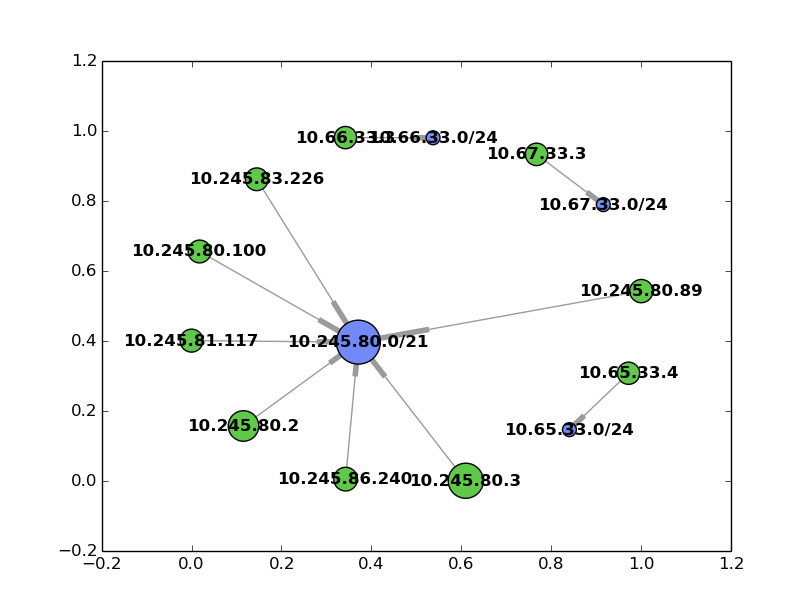
\includegraphics[scale=0.80]{imagenes/TCORP-wireless.png}

Puede verse en la componente conexa más grande del grafo que los nodos distinguidos más grandes son el 10.245.80.2 y 10.245.80.3, hipotetizamos de acuerdo a nuestro modelo que esos dos nodos juegan el papel de default gateway en la red. Sabemos también a priori que la ip del equipo que efectuó la captura es 10.245.80.89.

Nos llamó la atención que el equipo que efectua la captura no tenga interacción con los gateways, asi como tampoco el resto de los nodos distinguidos que aportan una cantidad de información similar a la capturadora. 

A lo largo de todo el desarrollo partimos del supuesto que los paquetes \textit{Who-has} eran la clave del modelado debido al principio teórico que manifiesta que todos los nodos actualizan sus tablas ARP utilizando paquetes de este tipo y siguiendo la idea que aquellos nodos que más actividad expresaban eran los default gateways dado que debían mantener información sobre toda la LAN, pero además sabemos que cada nodo debe actualizar la información sobre su default gateway de la misma manera, con lo que la ausencia de conexiones entre los equipos calificados como distinguidos con sus default gateways nos pareció una inconsistencia importante.

Indagando un poco más en la configuración de la capturadora, nos encontramos que por si esta inconsistencia no fuera suficiente, el default gateway que tenía configurada era un nodo que ni siquiera califica como distinguido, aquel cuya ip es 10.245.80.1 (que queda agrupado dentro de la nube de nodos no distinguidos). 

Llegados a este punto del análisis acudimos a metodologías experimentales y no tanto para arrojar más luz sobre la topología de la red, que pasamos a detallar.

Primero analizamos los datos arrojados por una fuente de información alternativa, particularmente, la fuente que distingue mensajes \textit{Who-has} basados en la ip destino. A pesar de las estrategias de agrupación de nodos y dimensionamiento en base a cantidad de información el gráfico generado es muy complejo para analizar a simple vista y decidimos no incluirlo, baste declarar que efectivamente aparece como nodo distinguido el default gateway declarado (10.245.80.1) pero su tamaño es sólo marginalmente mayor que el del resto de los nodos distinguidos hallados, y siendo estos notablemente más que para la fuente original, se dificulta hallarlo en una inspeción visual.\\

% Posterior al análisis experimental
Para complementar el análisis puramente experimental acudimos a enfoques alternativos tales como analizar los nodos distinguidos con otras herramientas, especificamente \textit{nmap} para verificar hipótesis sobre cuales eran los verdaderos gateways y cuales eran equipos normales que sólo calificaban como nodos distinguidos debido a su actividad excesiva en relación con los nodos no distinguidos. Basados en la detección de sistema operativo que ofrece, confirmamos que los nodos distinguidos 10.245.80.2 y 10.245.80.3 eran efectivamente elementos de red, dado que sus sistemas operativos eran \textit{Cisco iOS}, adicionalmente se confirmó que el resto de los nodos distinguidos dentro de la componente conexa que estamos analizando eran equipos de usuario final, en general con alguna variante de sistema operativo Windows y reforzados por los hostnames descubiertos que seguian la nomenclatura estricta de los equipos pertenecientes al dominio corporativo en la empresa. El análisis mediante nmap del default gateway declarado arrojó que el nodo no respondía con ninguna información útil.

La hipótesis a la que arribamos, luego de comentar la situación con expertos en el lugar de la captura, fue que probablemente la ip 10.245.80.1 perteneciera a un balanceador de carga /una especie de ip virtual) que distribuyera la misma entre dos nodos físicos: 10.245.80.2 y 10.245.80.3, esto explica tambien la ausencia de conexiones entre los nodos distinguidos que resultaron ser PCs de usuarios finales y los gateways descubiertos, dado que los paquetes \textit{Who-has} de estos nodos para actualizar la MAC de su default gateway fueron efectuados hacia la 10.245.80.1 (que queda oculta dentro de la nube) mientras que la actualización de las tablas ARP de los default gateways físicos, se generaba con origen ip de las ips físicas de dichos nodos.

Esto aún dejaba la duda de por qué los gateways físicos no actualizaban la información del resto de los nodos distinguidos, nuestra conclusión es que al experimentar mucho tráfico (el tráfico suficiente para que califique como nodo distinguido) y debido a la naturaleza asimetrica de la red en cuestión, la capturadora generó mucho trafico preguntando por su default gateway declarado 10.245.80.1 (que es una ip de balanceo descargando sobre 10.245.80.2 y 10.245.80.3  que como puede apreciarse por los tamaños de esos nodos en el grafico son aquellos nodos más distinguidos - aquellos con mayor actividad): la tabla ARP de los gateways resetea su tiempo de vida en relación al nodo que efectua la captura, haciendo innecesario que los gateways salgan a preguntar a toda la red, quien posee la dirección ip 10.245.80.89.
Similarmente arribamos a una conclusión paralela para el resto de los nodos distinguidos que registra menor actividad que los gateways.\\

También se confirmó esta hipótesis averiguando con los encargados del diseño, implementación y mantenimiento de la red, quienes verificaron que los gateways principales en la red eran los nodos 10.245.80.2 y 10.245.80.3 para la red de mayor actividad, que es a la que el equipo capturador se encontraba asociada (y adicionalmente aquella cuyo rango de potencia de radio era más fuerte debido a la cantidad de actividad mayor que se registró). También nos indicaron que por política de la empresa las primeras 15 ips disponibles de cada red se reservaban para la utilización a discreción del grupo de networking.

Pueden observarse superpuestas en el grafico redes de menor tamaño y trafico en los que la evidencia experimental (y la investigación de la infraestructura llevada a cabo) para lo que ocurre lo mismo: los gateways están dentro de los primeros 15 hosts de la red (reservados por el grupo de networking en todas las redes corporativas), en particular en los x.x.x.3 y x.x.x.4 y actualizan su tabla respecto de hosts que estan en sus redes (10.65.33.0/24, 10.66.33.0/24 y 10.67.33.0/24)

A continuación se presentan los resultados para las fuentes $S$ y $S1$ a nivel teoría de la información y entropía.

\begin{center}
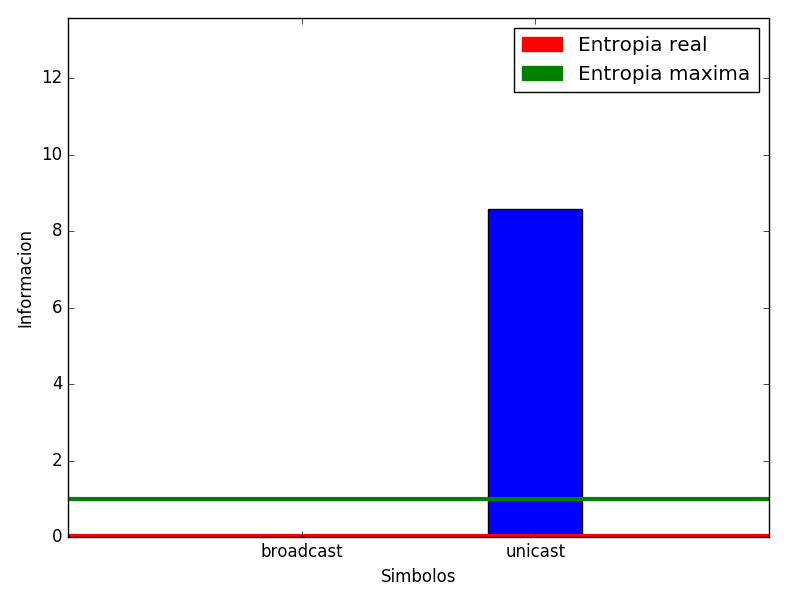
\includegraphics[scale=0.7]{imagenes/captura-tcorp-fuente-s.png} 
\end{center}

Puede verse que los broadcast superan en cantidad a los unicast: esto es, posiblemente, porque se capturan los broadcast de toda la red y sólo los unicast que están al alcance de radio del wi-fi. Es por esto que los unicast nos aportan tanta información.

\begin{center}
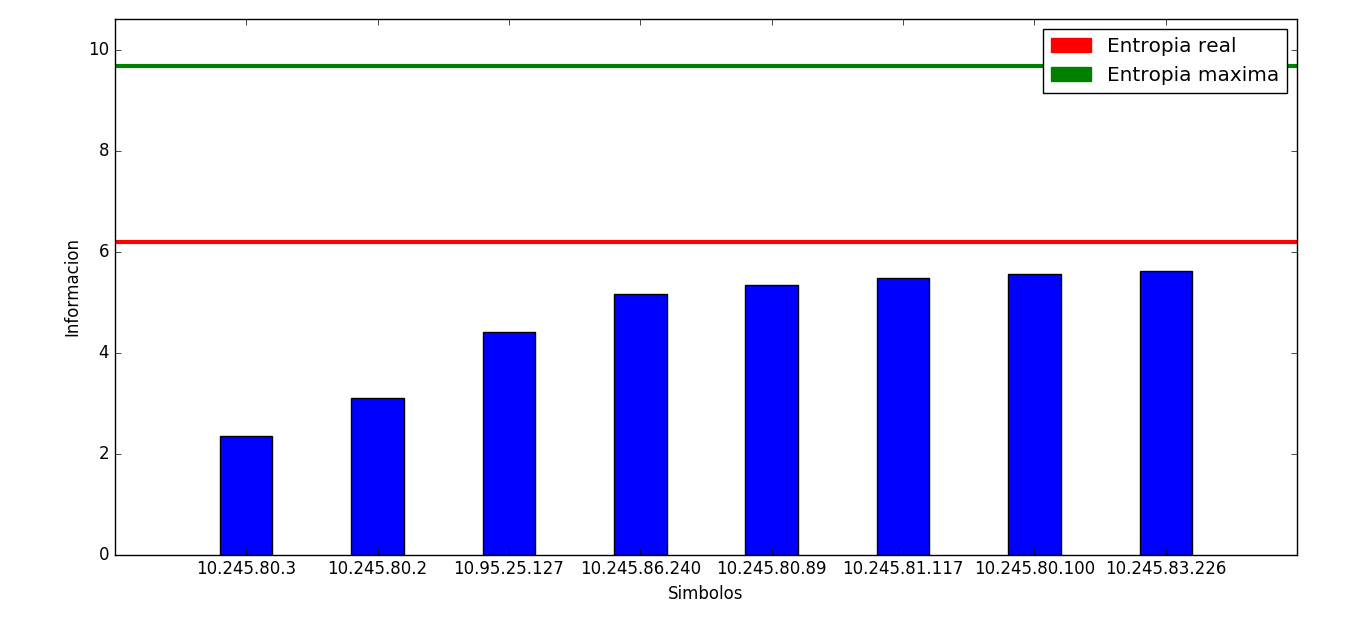
\includegraphics[scale=0.5]{imagenes/captura-tcorp-fuente-s1.png} 
\end{center}

Aquí puede verse que a medida que la información crece dentro de los nodos distinguidos, la curva se va suavizando, lo que creemos que indica que los nodos con mayor cantidad de información son de la misma naturaleza entre sí.
Luego, los nodos que aportan menor cantidad de información pueden distinguirse a partir del gráfico como los gateways, teniendo en cuenta el análisis previo.


\newpage

\subsection{Red corporativa mediana}

Esta es una red de la cuál conocemos la topología: consiste de un único router al cuál se conectan unas 30 pc's y una cantidad similar de celulares.


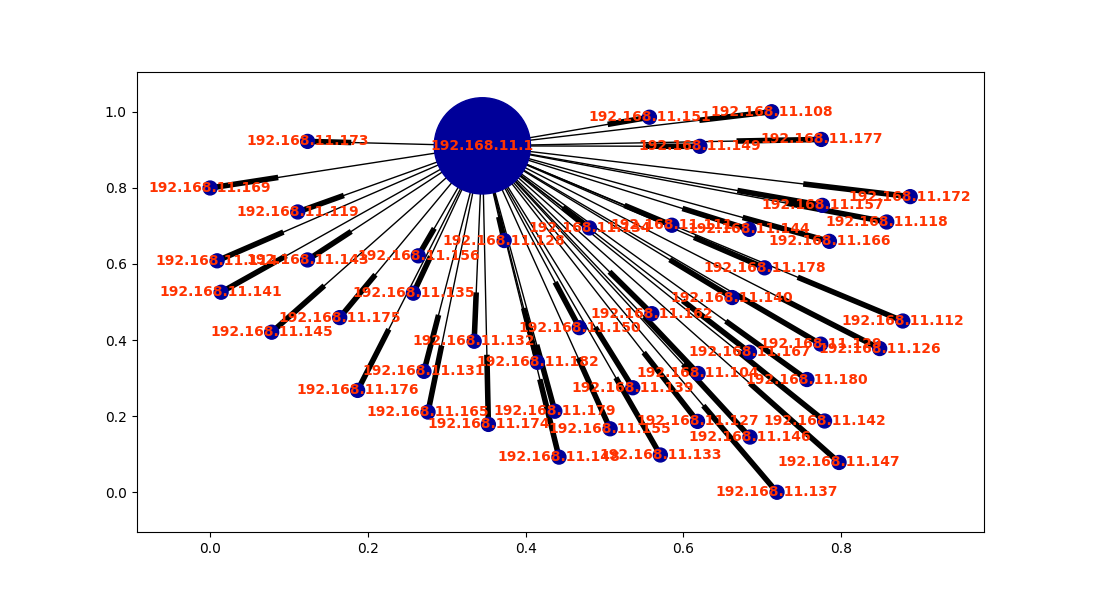
\includegraphics[scale=0.65]{imagenes/captura_red_trabajo_grafo.png}

Se puede ver que el default gateway (192.168.11.1), aparece como el nodo central al cual todo el resto de los nodos se conectan.

A continuación mostramos la entropía de las fuentes $S$ y $S1$ y la información de cada símbolo:

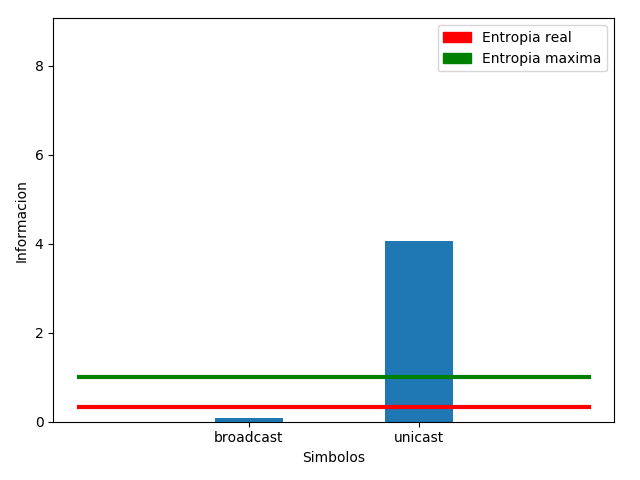
\includegraphics[scale=0.65]{imagenes/captura_red_trabajo_fuente_s.png}

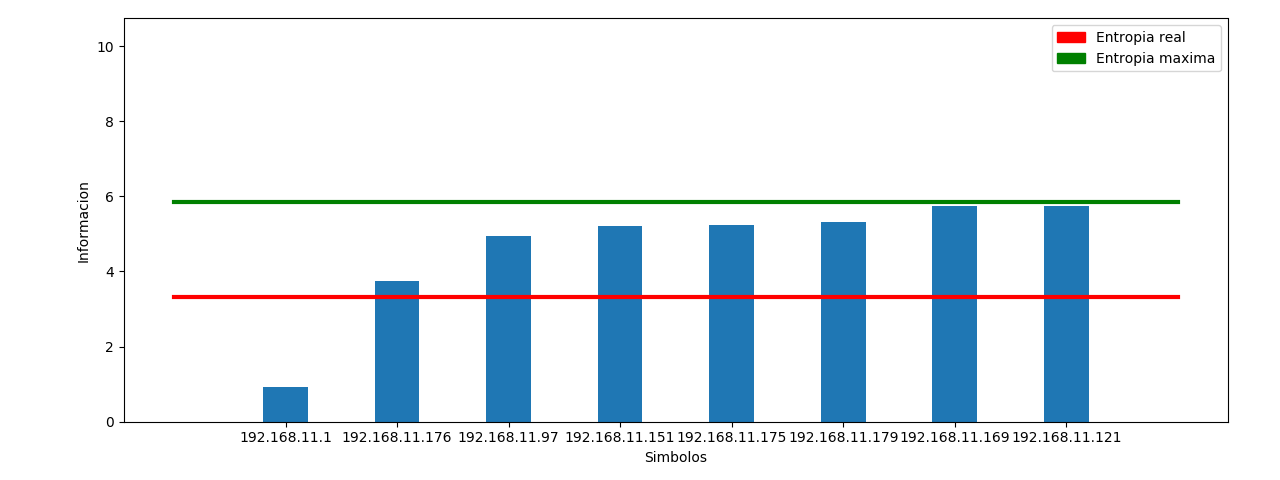
\includegraphics[scale=0.65]{imagenes/captura_red_trabajo_fuente_s1.png}

Tanto para $S$ como para $S1$ podemos observar que la entropía es menor que la entropía máxima. Sabemos que una fuente de memoria nula tiene entropía máxima cuando todos sus símbolos son equiprobables. Que la entropía real sea menor nos indica que hay ciertos símbolos más probables que otros. 

En el caso de la fuente $S$, en la captura observamos que el router está constantemente emitiendo paquetes \textit{Who-has}. Por lo tanto, observar el símbolo \textit{Broadcast} es altamente probable, lo cual implica que aporta muy poca información (0.0894 bits), mientras que el símbolo \textit{Unicast} aporta mucha más información (4.0557 bits), haciendo que \textit{Broadcast} sea un nodo distinguido, ya que la entropía de la fuente es 0.3279. La entropía máxima es 10.6995. Creemos que debido a que las tablas de ARP se deben refrescar cada cierto tiempo, la red experimenta un flujo mucho mayor de paquetes \textit{Broadcast} que \textit{Unicast}, dando lugar a una disparidad en la probabilidad de cada símbolo.

En el caso de la fuente $S1$, el único nodo distinguido que nos quedó fue el Default Gateway (pudimos comprobar empíricamente que este nodo lo era ejecutando el comando netstat -nr | grep default), indicando que la manera de seleccionar los símbolos que elegimos para esta fuente funciona muy bien con esta red. Al ser una red con una topología relativamente simple, no podemos asegurar que estos resultados se puedan extrapolar a redes más complejas. Algunos de los otros nodos, como 192.168.11.97 y 192.168.11.151, corresponden a otras notebooks conectadas a la red, lo cual nos resultó un comportamiento extraño. Suponemos que en esas notebooks se estaba ejecutando algún programa que trabaja a bajo nivel y está constantemente obteniendo información de la red local.

\newpage

\subsection{Red corporativa de empresa de Telecomunicaciones - Ethernet switcheada}
%1. ¿La entropía de la fuente S es máxima? ¿Que sugiere esto acerca de la red? ¿Está relacionado con el
%overhead impuesto por la red debido a los protocolos de control (i.e.: ARP)?
\textbf{Datos obtenidos con la fuente $S$:}

\begin{center}
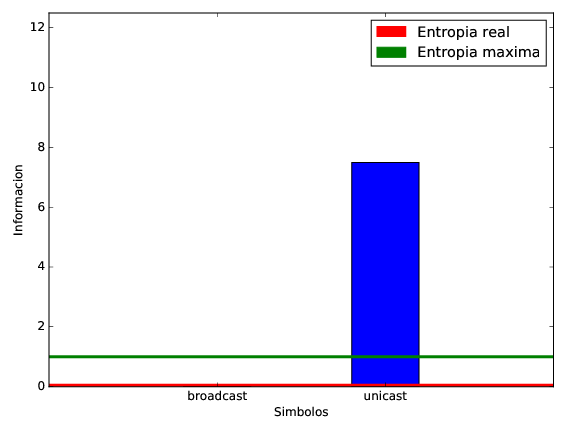
\includegraphics[scale=0.6]{imagenes/analisisTCORPcableada/fuenteS.png} 
\end{center}

Como se puede observar hay muchísimos más broadcast que unicast, es por ello que el último dá más información. Las probabilidades son las siguientes: broadcast 0.99, unicast 0.01. La entropía es 0.049, casi nula.\\

Los broadcast son visibles para todos los dispositivos, mientras que los unicast no. Al ser una red switcheada, nosotros estamos viendo los broadcast de todos los hosts y sólo nuestros unicast (respuestas enviadas al host con el cuál se hizo la captura), es por esto que la diferencia es tan grande.\\

%2. ¿Cómo es el tráfico ARP en la red? ¿Se pueden distinguir nodos? ¿Cuántos? ¿Indica algo la cantidad?
%¿Se les puede adjudicar alguna función específica? ¿Hay evidencia parcial que sugiera que algún nodo
%funciona de forma anómala y/o no esperada?
%3. ¿Existe una correspondencia entre lo que se conoce de la red y los nodos distinguidos detectados por
%la herramienta? ¿Es posible usar el criterio de distinción propuesto como método para descubrir el/los
%Default Gateway/s de la red? ¿Es preciso?
\textbf{Datos obtenidos con la fuente $S1$:}

\begin{center}
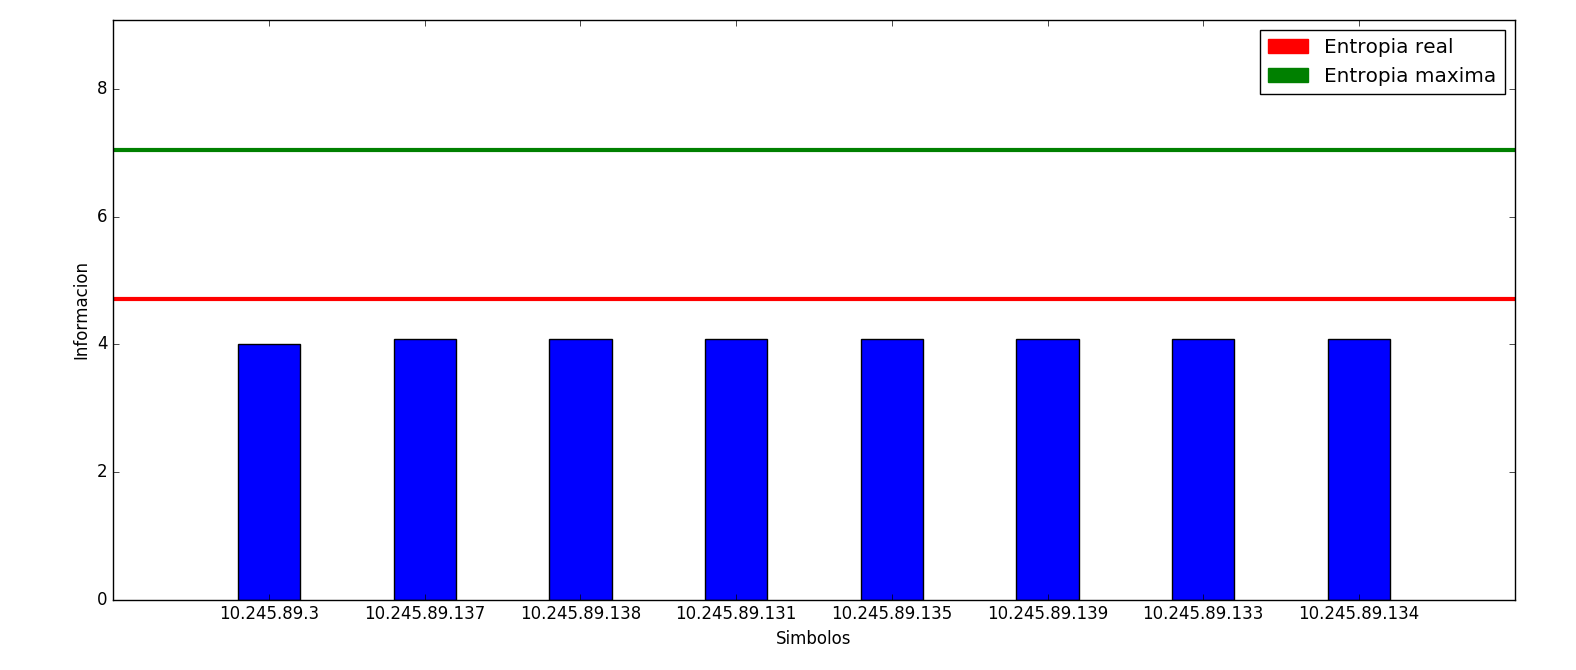
\includegraphics[scale=0.4]{imagenes/analisisTCORPcableada/fuenteS1-11.png} 
\end{center}

Observando la disposición de la red descubrimos manualmente que posee dos IP físicas de gateways, 10.245.89.3 y 10.245.89.2 y una IP que actúa como balanceador, 10.245.89.1, a la cuál los hosts realizan sus pedidos y ésta los redirecciona a 10.245.89.3 o 10.245.89.2 según la carga de cada uno.

\begin{center}
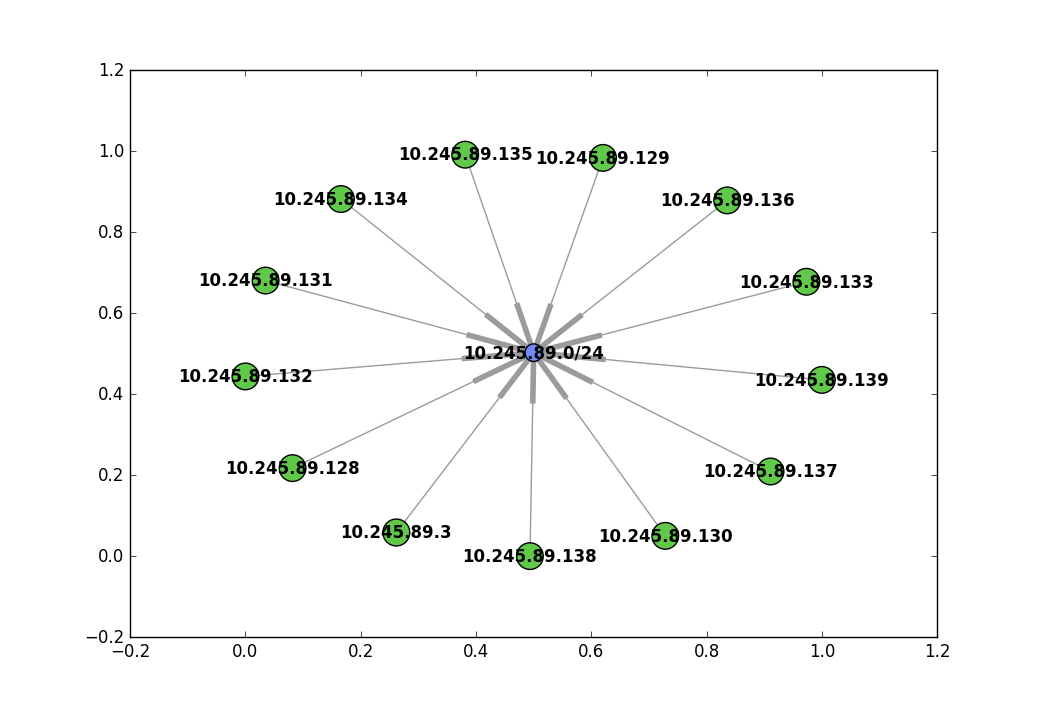
\includegraphics[scale=0.65]{imagenes/analisisTCORPcableada/cableada-11sum.png} 
\end{center}
\vspace*{-1cm}

Los nodos distinguidos que vemos en el gráfico son hosts con mucha actividad, los cuáles están consultando a 10.245.89.1. Quien se encuentra incluído en la red ya que recibe pedidos pero las respuestas a estos son emitidas por 10.245.89.3 o 10.245.89.2 entonces no llega a ser distinguido si nuestros símbolos son los IP de origen.

Dentro de estos nodos distinguidos también se encuentra una de los IP físicas de los gateways, 10.245.89.3. Quién queda ocluído por la actividad de los demás equipos.\\

Como no obtuvimos buenos resultados a la hora de detectar el default gateway, probamos con otra fuente a la cuál llamaremos $S2$, que tiene como símbolos los IP destino de los paquetes ARP Who-Has.\\

Para esta nueva fuente los datos obtenidos son los siguientes:
\begin{center}
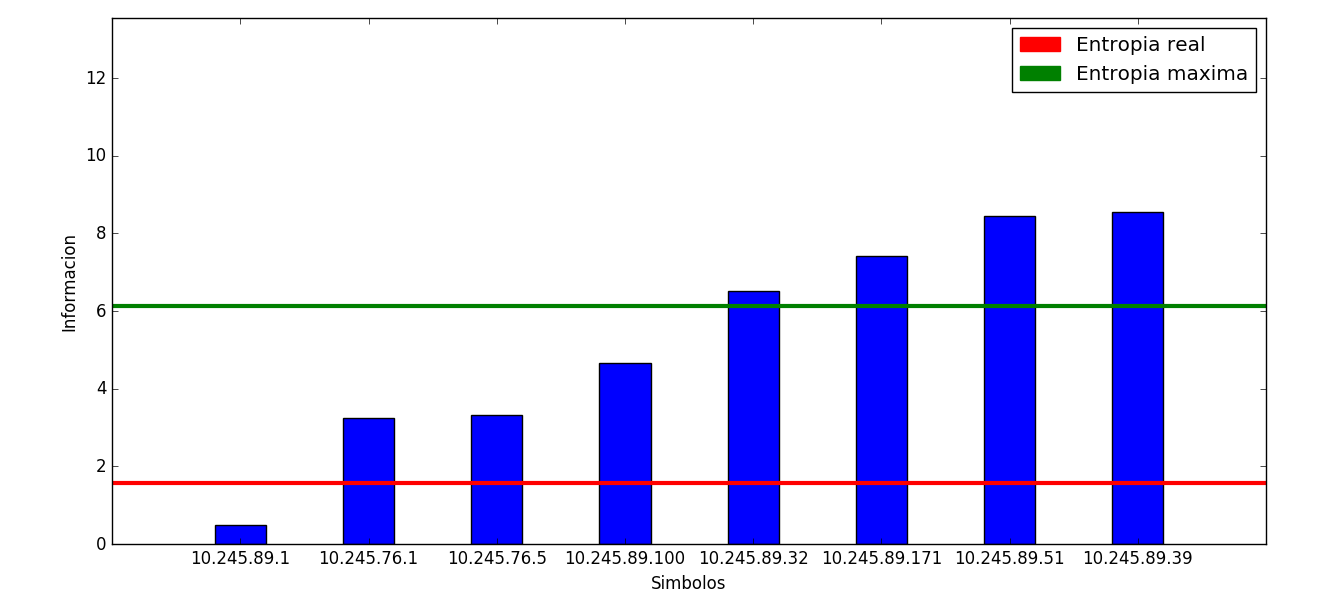
\includegraphics[scale=0.5]{imagenes/analisisTCORPcableada/fuenteS1-12.png} 
\end{center}

En este caso hay un solo nodo distinguido. El cuál, como vimos antes, es el balanceador. Éste es el default gateway para toda la red, quien se encarga de redirigir los pedidos.\\

Todos los equipos en la Lan preguntan la MAC del default gateway para actualizar sus tablas, lo hacen mediante broadcast a nivel de enlace con lo cual el paquete lo ven todos los nodos en dominio de broadcast, en particular la maquina con la que efectuamos la captura.\\

El motivo por el cuál funciona mejor la fuente $S2$ que la $S1$ en este caso, suponemos que se debe tanto al tipo de conexión (ethernet switcheada) como a la disposición (i.e. el hecho de que tenga un balanceador distinto de las IP físicas de los gateways).

\begin{figure}[htbp]
\hspace*{-2cm}                                                           
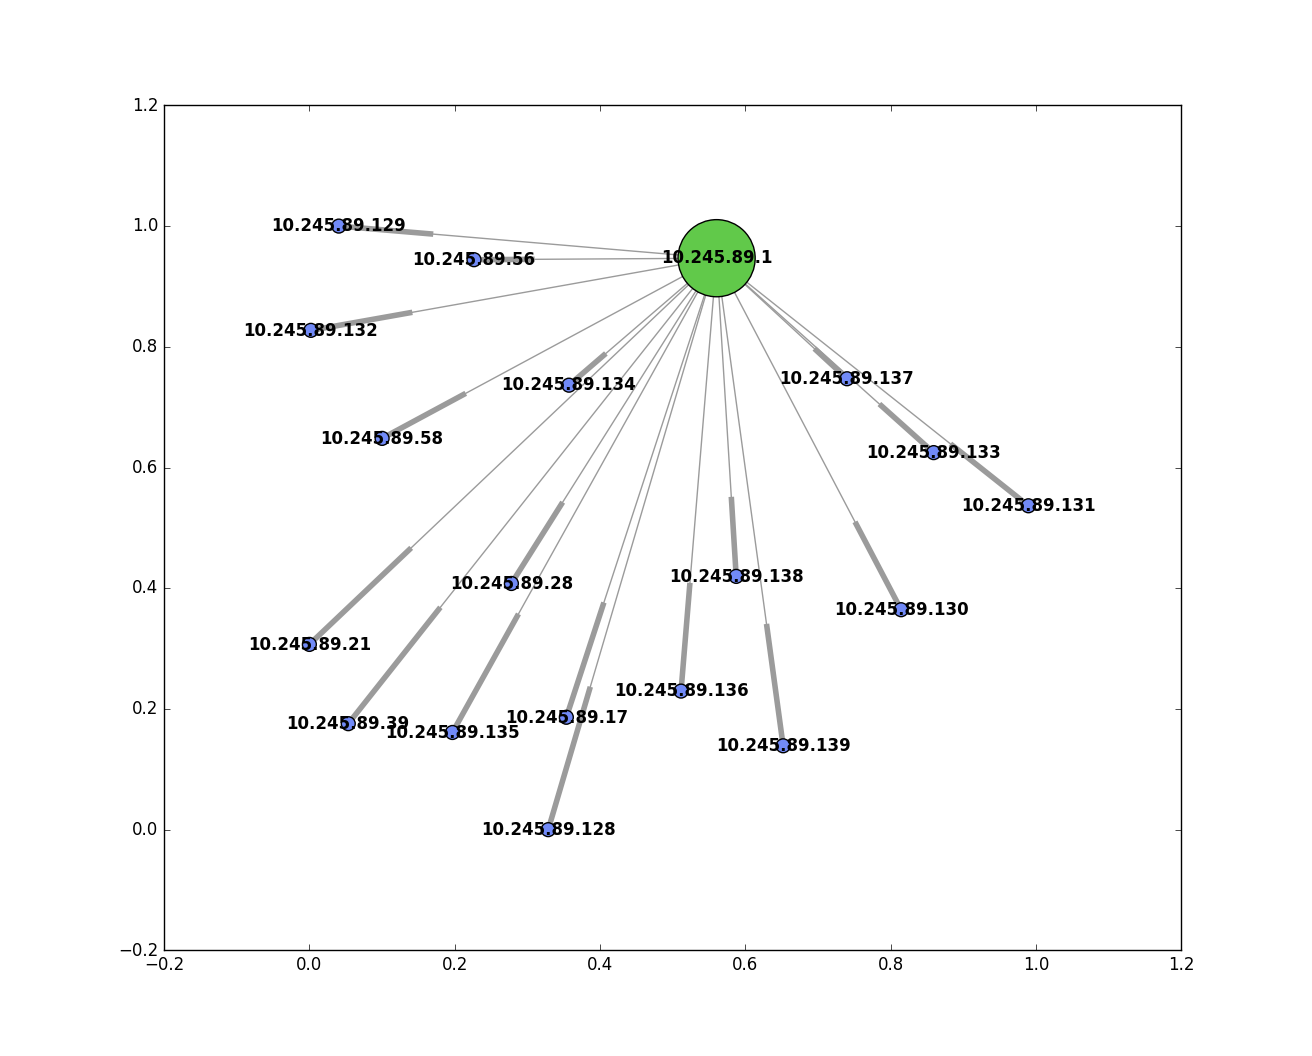
\includegraphics[scale=0.6]{imagenes/analisisTCORPcableada/cableada-12.png} 
\end{figure}








\newpage

\subsection{Red doméstica - wireless LAN}
Esta captura se realizó a partir de una red doméstica, con dos computadoras conectadas por cable ethernet y varios dispositivos wireless (laptops, celulares, impresora y chromecast).

\textbf{Fuente S}:

La entropía obtenida (aproximadamente 0.924) se acerca bastante a la máxima, a diferencia de las otras capturas que poseen una entropía muy baja. Además como se observa en el gráfico, la proporción de mensajes unicast fue mayor que la de broadcast.	

\begin{figure}[H]
\centering
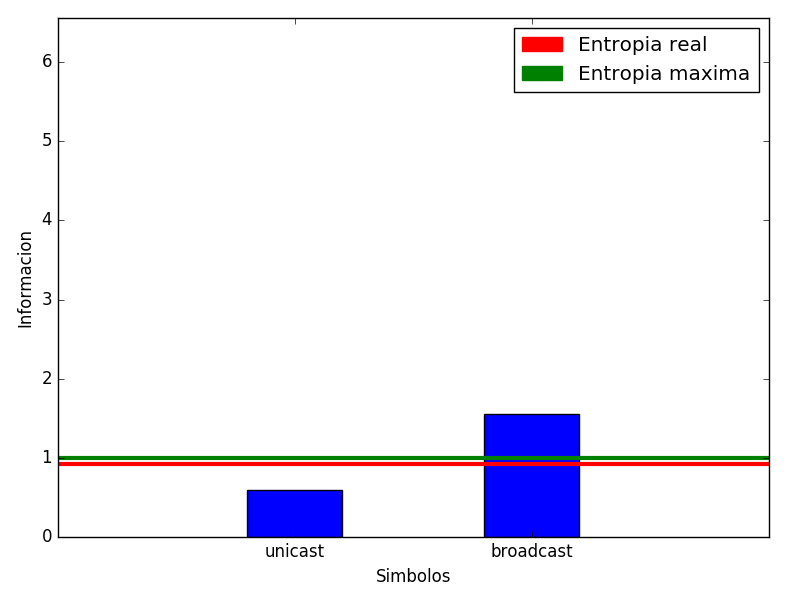
\includegraphics[keepaspectratio=true,scale=1,width=1\linewidth]{imagenes/red-dom-S}
\caption{Red doméstica - Fuente S}
\label{fig:red-dom-S}
\end{figure}

Todo este comportamiento se debe a que al haber pocos dispositivos dentro de la red y tratándose siempre de los mismos, las tablas ARP de cada nodo se mantienen más estables (menos probabilidad de anomalías) y los mensajes broadcast se observan con menos frecuencia.

\textbf{Fuente S1}:

El análisis a partir de S1 (no se agruparon nodos por tratarse de una red pequeña), muestra un único nodo distinguido que coincide con el default gateway de la red (192.168.0.1).

\begin{figure}[H]
	\centering
	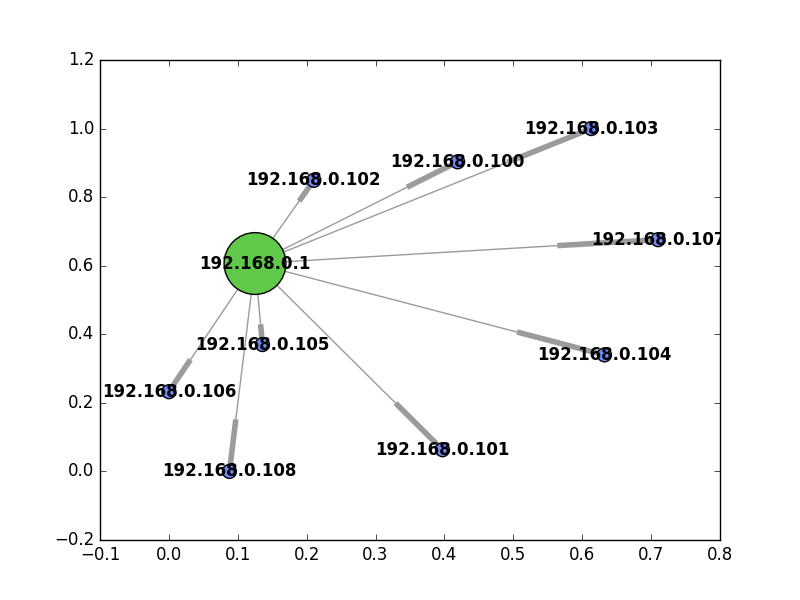
\includegraphics[width=0.8\linewidth]{imagenes/grafo-red-luis.png}
	\caption{Grafo derivado de S1 }
	\label{fig:eth-red-domestica}
\end{figure}

Para tener un análisis más detallado generamos el grafo con las mismas condiciones que antes pero agregando las conexiones entre nodos no distinguidos.

\begin{figure}[H]
	\centering
	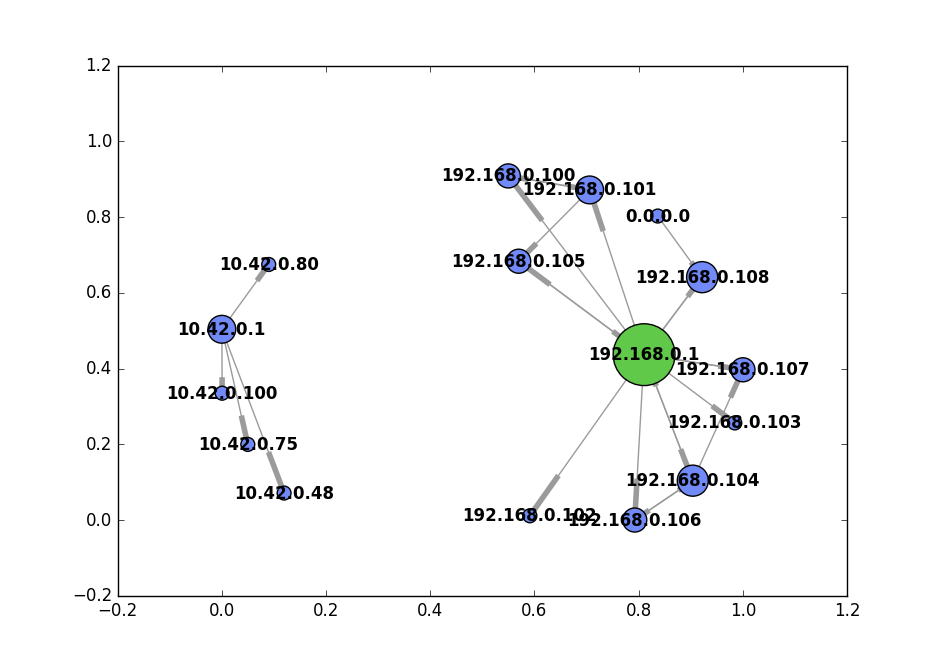
\includegraphics[width=0.8\linewidth]{imagenes/grafo-full-redLuis}
	\caption{Grafo con conexiones de nodos no distinguidos}
	\label{fig:grafo-full-redLuis}
\end{figure}

Se observan dos puntos interesantes:
 \begin{itemize}
 	\item El primero es la aparición de un nuevo conjunto de nodos que aparentemente forman una red, este tráfico corresponde a paquetes broadcast que son capturados ya que la traza fue realizada en "modo promiscuo", es decir, capturando todo el tráfico que la tarjeta de red puede "ver".
 \item El segundo es la aparición de un nodo con IP "0.0.0.0'', analizando en detalle la traza nos dimos cuenta que se trataba de un paquete broadcast ''Who-has'' enviado por un dispositivo que intentaba conectarse por primera vez a la red, al principio no posee IP, por eso está con el valor nulo "0.0.0.0", pregunta por cierta IP (192.168.0.108), que es la que intentará utilizar desde ese momento, como no está asignada se la adjudica a través de un \textit{Gratuitous ARP}, que básicamente sirve para anunciar a la red que IP está utilizando. Además este dispositivo tiene una interacción bastante frecuente con el default gateway.
 \end{itemize}
 
La entropía de la fuente es aproximadamente la mitad de la  máxima, el default gateway es el que menos información aporta, seguido por el nodo que obtiene la IP 192.168.0.108 mencionado anteriormente, el default gateway de la red externa capturada por la traza y el nodo con IP 192.168.0.104 que corresponde a una impresora. El resto de los nodos son los que aportan más información (símbolos con menor frecuencia).

\begin{figure}[H]
\centering
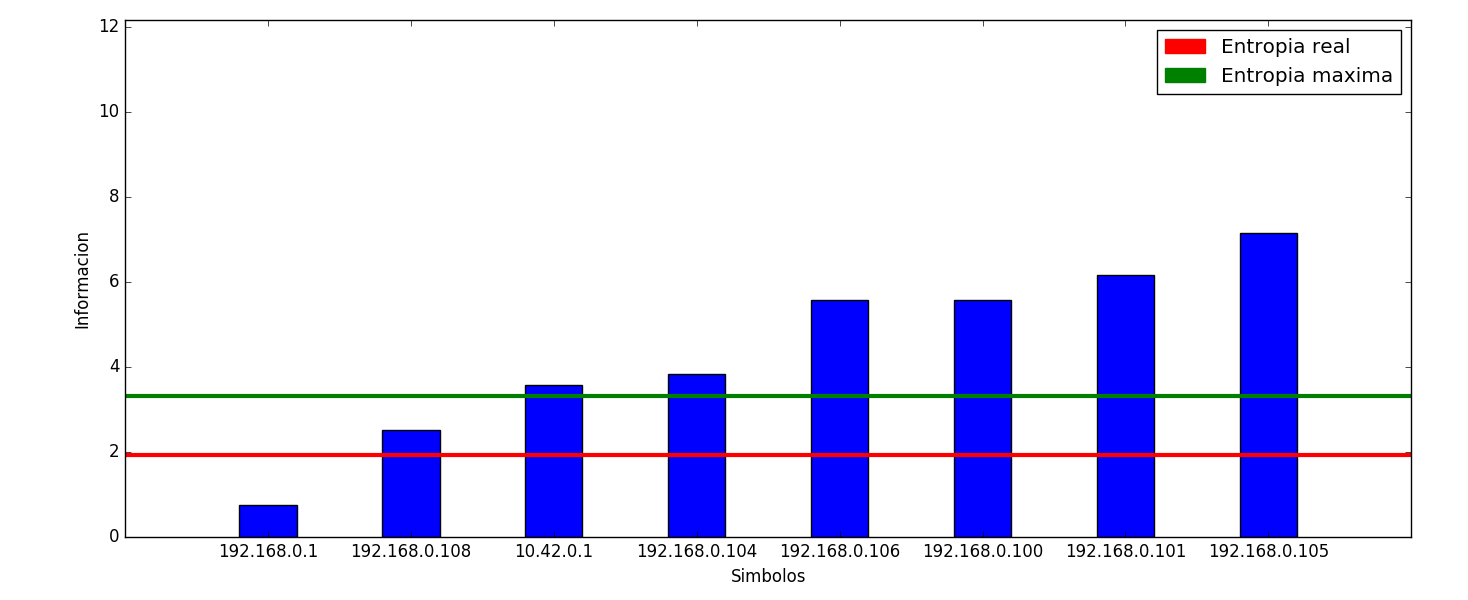
\includegraphics[width=0.8\linewidth]{imagenes/red-dom-S1}
\caption{}
\label{fig:red-dom-S1}
\end{figure}

En este caso la detección de nodos distinguidos parece ser bastante precisa para detectar default gateways, a pesar que se escucha tráfico de otras redes.
\newpage
	\newpage
	
	\section{Conclusiones}



\addtolength{\textheight}{-12cm}   % This command serves to balance the column lengths
% on the last page of the document manually. It shortens
% the textheight of the last page by a suitable amount.
% This command does not take effect until the next page
% so it should come on the page before the last. Make
% sure that you do not shorten the textheight too much.



%%%%%%%%%%%%%%%%%%%%%%%%%%%%%%%%%%%%%%%%%%%%%%%%%%%%%%%%%%%%%%%%%%%%%%%%%%%%%%%%
	\newpage
	
	\section{Referencias}

\begin{enumerate}

\item 
\url[1] {http://www.secdev.org/projects/scapy/}
\item[2] \url{http://www.wireshark.org}

\end{enumerate}

	\newpage
	
	\bibliographystyle{plain}
	\bibliography{tp3}
	
\end{document}



\begin{document}

\maketitle
\thispagestyle{empty}
\pagestyle{empty}


%%%%%%%%%%%%%%%%%%%%%%%%%%%%%%%%%%%%%%%%%%%%%%%%%%%%%%%%%%%%%%%%%%%%%%%%%%%%%%%%
\begin{abstract}
En el presente trabajo se utilizan la libreria Scapy de Python y la herramienta Wireshark para capturar paquetes ARP en varias redes y modelar dos fuentes de memoria nula. Sobre estas fuentes se efectúa un análisis de la entropía de cada una de ellas y de la cantidad de información que transmite cada símbolo de estas fuentes. Adicionalmente se busca verificar qué datos de la topología de las redes subyacentes pueden descubrirse en base a los símbolos distinguidos de estas fuentes y ayudar a la profundización del conocimiento sobre el protocolo ARP en escenarios reales.
\end{abstract}
\keywords{ARP, Scapy, Wireshark, Entropía, Fuentes de memoria nula, Cantidad de información, Topología de redes en capa 2.}


\section{Conclusiones}



\addtolength{\textheight}{-12cm}   % This command serves to balance the column lengths
                                  % on the last page of the document manually. It shortens
                                  % the textheight of the last page by a suitable amount.
                                  % This command does not take effect until the next page
                                  % so it should come on the page before the last. Make
                                  % sure that you do not shorten the textheight too much.



%%%%%%%%%%%%%%%%%%%%%%%%%%%%%%%%%%%%%%%%%%%%%%%%%%%%%%%%%%%%%%%%%%%%%%%%%%%%%%%%

\begin{thebibliography}{99}

\bibitem{c1} http://www.wireshark.org
\bibitem{c2} http://www.secdev.org/projects/scapy/

\end{thebibliography}

\end{document}
